\chapter{Техническая реализация}
\label{sec:chap3}

\section{Описание реализации}

\subsection{Первая версия}

\begin{figure}[!h]
\centering
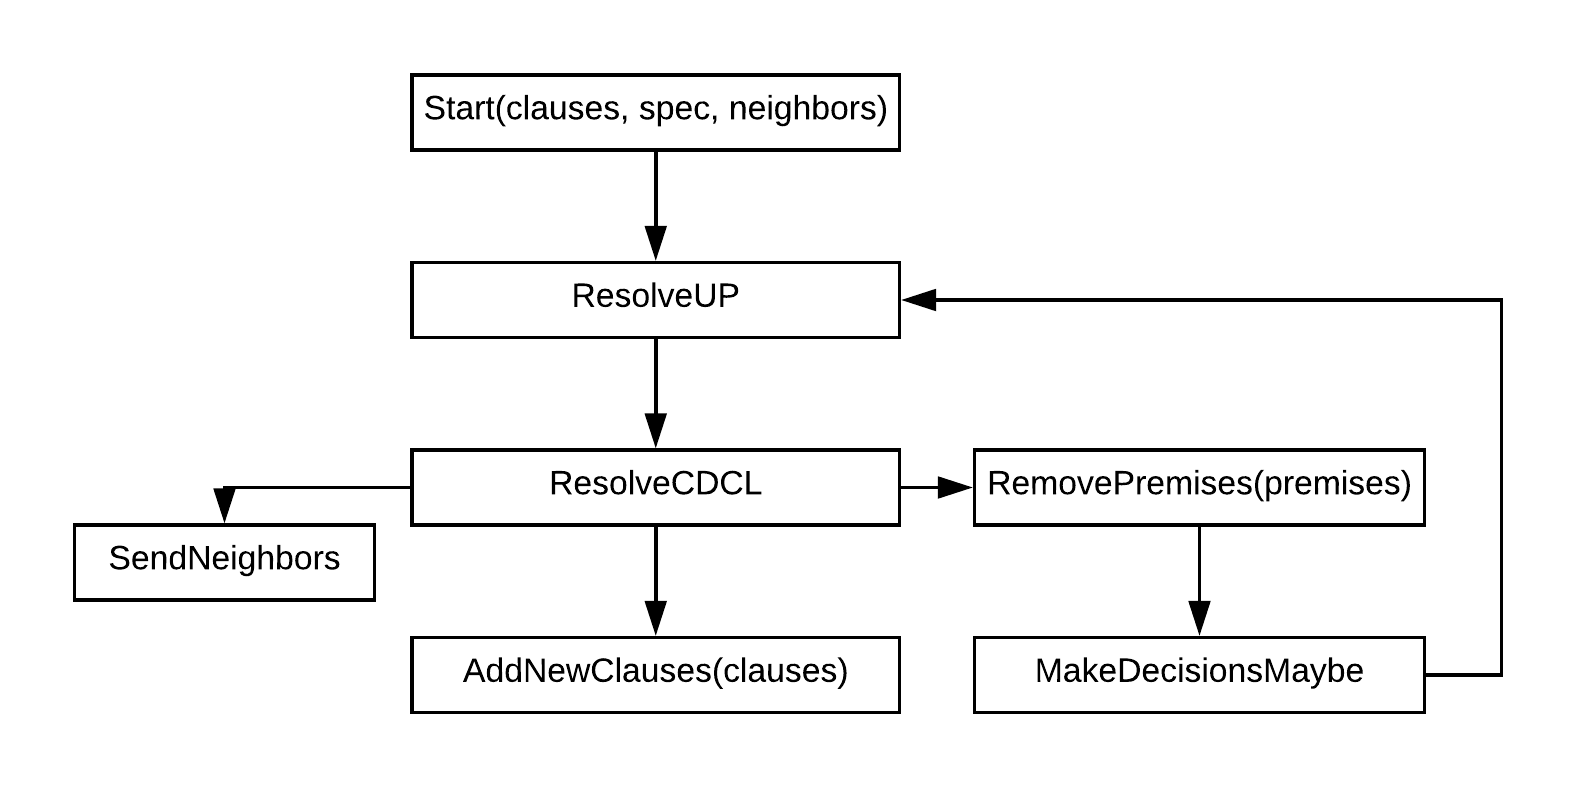
\includegraphics[scale=0.9]{actorProcess.png}
\caption{Сообщения внутри одного актора.}\label{fig:actorProcess}
\end{figure}

На рисунке \ref{fig:actorProcess} описано то, как ведёт себя один актор, для случая статической специализации.
Изначально мы посылаем каждому актору все сообщения с помощью тега \emph{Start}.
\begin{lstlisting}[language=scala]
    case Start(initialClauses, actors) =>
      onReceiveStart(initialClauses, actors)
      self ! ResolveUnitPropagation
\end{lstlisting}

Далее выполняется поиск резолюций -- для этого перебирается клоз, выбирается один литерал, для остальных же ищем соответствующую пару в структуре данных, поддерживающей поиск унифицирующих литералов. Далее применяем унификатор к выбранному литералу, и добавляем его в базу данных внутри этого актора.

После стадии поиска резолюций, начинается выявление конфликтов. Для поиска конфликтов мы должны перебрать пару литералов, где хотя бы один был выведен на последней итерации, и попытаться подобрать унификатор. Если это получилось, то мы нашли локальный конфликт. В локальном конфликте мы должны проверить существование предположений. Если они есть, то применить правило \emph{CDCL}. Если же их нет, то мы должны взять остаточный клоз и разослать его всем соседям в нашей топологии. Если остаточный клоз тоже пустой, то мы нашли конфликт и необходимо завершить работу всех акторов.

Если на последней итерации стадий \emph{CDCL} и \emph{Unit-Propagation Resolution} не было выявлено новых литералов, то нам нужно сделать предположение. Выбор предположений -- отдельная очень обширная для изучения тема, в которой можно использовать методы обучения с подкреплением, различные простые эвристики. Однако, в рамках данной реализации предположение выбирается случайным образом.

\subsection{Проблема реализации и её решение}
\begin{figure}
  \begin{prooftree}
      \def\defaultHypSeparation{\hskip .1in}

                      \AxiomC{$[A]^1_1$}
                      \AxiomC{$\neg A \vee D$}
                    \RightLabel{$\confl{1}{}$}
                  \BinaryInfC{$D^1$}
                \RightLabel{$\kshare{1}{2}$}
              \UnaryInfC{$D^2$}

                        \AxiomC{$[A]^1_1$}
                        \AxiomC{$\neg A \vee C$}
                      \RightLabel{$\confl{1}{}$}
                    \BinaryInfC{$C^1$}
                  \RightLabel{$\kshare{1}{2}$}
                \UnaryInfC{$C^2$}
                \AxiomC{$\neg C \vee \neg D$}
                \RightLabel{$\upr{2}{}$}
              \BinaryInfC{$(\neg D)^2$}

              \RightLabel{$\confl{2}{}$}
             \BinaryInfC{$\bot$}
             \RightLabel{$\cdcl{2}{1}$}
             \UnaryInfC{$(\neg A)^2$}
  \end{prooftree}
  \caption{Пример на \emph{CDCL} (вывод $\neg A$)}
  \label{fig:example-cdcl-1}
\end{figure}



\begin{figure}
  \begin{prooftree}
    \def\defaultHypSeparation{\hskip .0mm}
        \AxiomC{$\alpha (= B^1)$}
        \AxiomC{$\neg B \vee D$}
        \RightLabel{$\confl{1}$}
      \BinaryInfC{$D^1$}
      \RightLabel{$\kshare{1}{2}$}
    \UnaryInfC{$D^2$}
    
             \AxiomC{$\infer[]{(\neg A)^2}{
               \text{(вывод из рис. \ref{fig:example-cdcl-1})}}$
             }
             \RightLabel{$\kshare{2}{1}$}
            \UnaryInfC{$(\neg A)^1$}
            \AxiomC{$(A \vee B)^1$}
            \RightLabel{$\upr{1}{}$}
          \BinaryInfC{$(\alpha = )B^1$}

          \AxiomC{$\neg B \vee C$}
          \RightLabel{$\confl{1}{}$}
        \BinaryInfC{$C^1$}
        \RightLabel{$\kshare{1}{2}$}
        \UnaryInfC{$C^2$}

	    \AxiomC{$\neg C \vee \neg D$}
      \BinaryInfC{$\neg D$}
    
	\BinaryInfC{$\bot$}
  \end{prooftree}
  \caption{Пример на \emph{CDCL} (вторая часть)}
  \label{fig:example-cdcl-2}
\end{figure}

\begin{example}
\label{exmpl:cdcl-fail}
Рассмотрим пример, показанный на рисунках \ref{fig:example-cdcl-1} и \ref{fig:example-cdcl-2}. Здесь находится противоречие для следующего набора формул: \begin{gather*}
			\{ A \vee B
             , \neg A \vee C
             , \neg A \vee D
             , \neg B \vee C
             , \neg B \vee D
             , \neg C \vee \neg D
            \}
		\end{gather*}
 Доказательство ищется в системе из двух акторов, со следующей специализацией $\Psi_1 = \{A, B\}$, $\Psi_2 = \{C, D\}$. Так как все клозы состоят по крайней мере из двух литералов, то нам придётся хотя бы раз воспользоваться правич]лом \emph{Conflict-Driven Clause Learning}. Проблема этого примера заключается в том, что предположение из одного актора даст нам конфликт в другом акторе, т.е. если мы будем делать \emph{CDCL} только внутри акторов, то наше исчисление не будет полным.
\end{example}

Заметим, что в такой реализации предположения не пересылаются между акторами, и правило \emph{CDCL} может выводить только клозы, состоящие из специализации актора. К сожалению, данной реализации недостаточно, чтобы сохранить полноту. Не составит труда понять, что для набора клозов из примера \ref{exmpl:cdcl-fail} не существует модели, опровергающей этот набор. 

Для решения этой проблемы будем использовать подход, похожий на архитектуру Нельсона-Оппена \ref{TODO} для задач о выполнимости формул в теориях (\emph{SMT}-решатели): актор $a$ может послать актору $b$ конъюнкцию литералов, и если $b$ нашёл конфликт, то сообщает об этом $a$, после чего $a$ делает соответствующие откаты.

Для реализации такого подхода, будем хранить в каждой вершине дополнительную информацию: список предположений, которые используются.

\section{Топология}
\begin{figure}[!h]
\centering
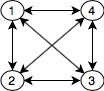
\includegraphics[scale=0.9]{Complete.png}
\caption{Каждый актор шлёт сообщения каждому.}\label{fig:complete}
\end{figure}

\begin{figure}[!h]
\centering
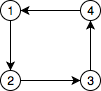
\includegraphics[scale=0.9]{Ring.png}
\caption{Актор посылает сообщение соседу слева}\label{fig:ring}
\end{figure}

Система акторов формирует топологию. Были протестированы два вида реализации: кольцо(рис. \ref{fig:ring}) и полный граф(рис. \ref{fig:complete}). Алгоритм с топологией в виде кольца назовём \emph{EAR}, а с топологией полного графа --- \emph{EAC}. 

На первый взгляд может показаться, что топология полного графа будет иметь плохую производительность, однако стоит заметить, что каждый отдельный актор решает NP-трудную задачу за экспоненциальную сложность, а количество сообщений от одного актора другому не так велико на практике, чтобы иметь значительный вес в оценке производительности.

\section{Доказательство полноты}
Для того, чтобы понять, что реализация работает, необходимо показать, что если существует вывод некоторой формулы в исчислении \emph{Expertised Conflict Resolution}, то какое-то доказательство найдётся и нашим алгоритмом. 

\begin{theorem}
Пусть существует некоторый вывод формулы $\phi^i$ в исчислении \emph{ECR}. Тогда алгоритм \emph{EAC} найдёт это доказательство за конечное время.
\end{theorem}
\begin{proof}
Будем доказывать по структуре графа доказательства в \emph{ECR}.
\begin{enumerate}[label=$\star$]
	\item \emph{База.} Вершина без входящих в неё рёбер. В такой вершине записан начальный клоз в виде $\xi^i$. Это означает, что актор $i$ специализируется на литерале $\xi$. И мы отправим ему сообщение $Start$, в котором будет содержаться выражение $\xi$.
    \item \emph{Переход.} Вершина получена одним из четырёх правил вывода: 
    \begin{enumerate}
      \item \emph{Unit-Propagation Resolution.} Если в \emph{ECR} вывод $\xi^i$ заканчивается применением правила \emph{Unit-Propagation Resolution} в акторе $i$, то этот актор найдёт применение правила, посколько он перебирает все возможные варианты. 
      \item \emph{Conflict.} Посколько на стадии \emph{ResolveConflicts} актор находит все возможные варианты конфликтов, а по предположению индукции все предпосылки уже выведены, то данное применение правила тоже будет найдено.
      \item \emph{Conflict-Driven Clause Learning.}
      \item \emph{Knowledge Sharing.}
    \end{enumerate}
\end{enumerate}
\end{proof}

% \section{Оценка сложности для задачи \emph{Принцип Дирихле}}
% В резолюционном исчислении сложно оценивать сложность общего алгоритма, поэтому чаще всего оценивается на конкретных задачах. Одной из таких классических задач является \emph{Принцип Дирихле}. 
% \texttt{TODO: написать здесь доказательство оценки}
\section{Оценка производительности}
\begin{figure}[!h]
\centering
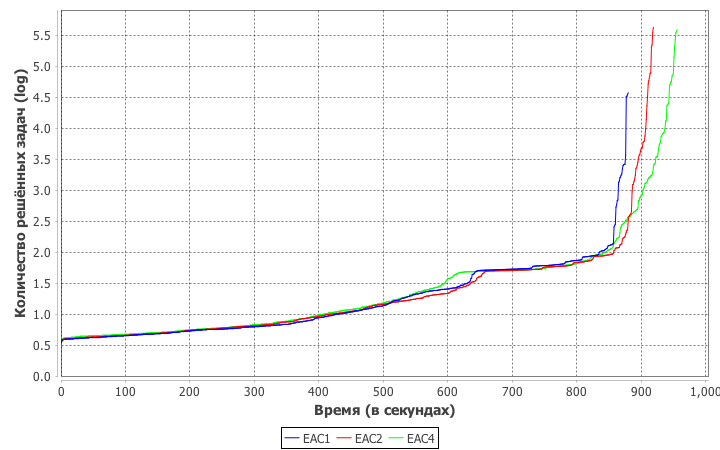
\includegraphics[scale=0.4]{chart.png}
\caption{График работы.}\label{fig:chart}
\end{figure}

На рисунке \ref{fig:chart} показана производительность реализации для $1$, $2$, и $4$ акторов. Для удобства по оси "количества решённых задач" была взята логарифмическая шкала. Версия решения с одним актором примерно соответствует алгоритму \emph{EPCR} \cite{DBLP:journals/corr/ItegulovSP17}, который основан на чистом исчислении \emph{Conflict Resolution}. Версия с одним актроом успела за 300 секунд найти опровергающие модели для 880 задач из 1606 доступных в архиве \emph{TPTP}. Для двух акторов -- 919 задач. Для четырёх -- 946.

\section{Выводы к третьей главе}
\begin{enumerate}
	\item Описан алгоритм на основе исчисления из главы \ref{sec:chap2}
    \item Доказана его полнота по опровержению
    \item Показана его производительность
\end{enumerate}